\section{Durchführung}
\label{sec:Durchführung}

Der prinzipielle Versuchsaufbau ist in Abbildung \ref{fig:aufbau} dargestellt. Die Alphastrahlung aus der 241-Americium-Quelle wird kollimiert. Die darauffolgende Folie kann ein- oder ausgebaut werden, um auch Studien der Reichweite von Alphastrahlung in Luft ohne Target durchzuführen. Der auf einer Schiene bewegliche Detektor ist ein Surface-Barrier-Detektor, der im Grunde einer Diode in Sperrrichtung entspricht.
In einem p-n-Übergang bildet sich eine Verarmungszone, in der durch einfallende Strahlung Elektronen-Loch-Paare entstehen. Diese werden durch das vorherrschende elektrische Feld, das durch die Sperrspannung hervorgerufen wird, zu den Elektroden hin abgesaugt und erzeugen einen messbaren elektrischen Impuls, der durch einen Verstärker noch weiter verstärkt werden kann. Das verstärkte Signal wird dann auf ein Speicheroszilloskop gegeben. Es ist auch möglich, einen Counter anzuschließen, um die Zahl der Alphateilchen, die den Detektor erreichen, zu messen.

\begin{figure}
  \centering
  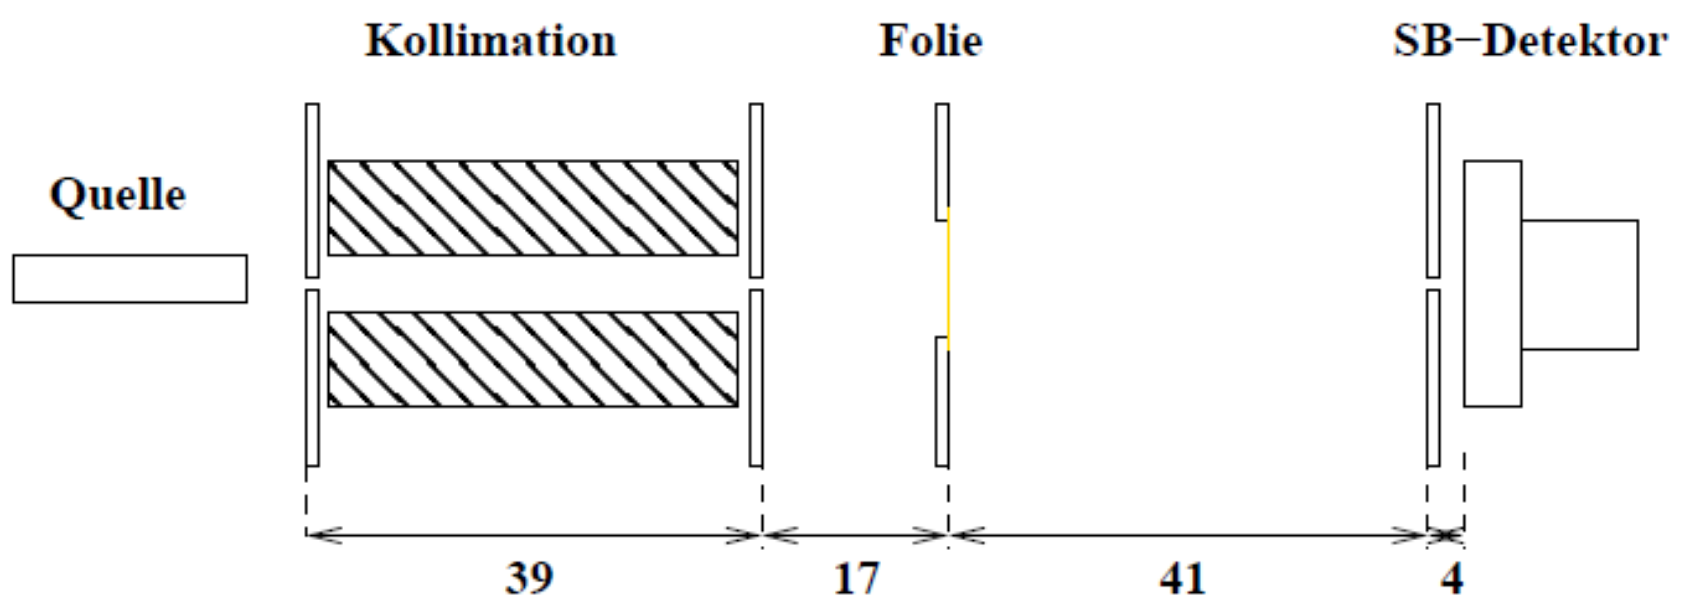
\includegraphics[width=\textwidth]{images/aufbau.png}
  \caption{Schematische Darstellung des Versuchsaufbaus mit seinen Abmessungen \cite{Versuchsanleitung}.}
  \label{fig:aufbau}
\end{figure}

Der Aufbau kann durch eine sogenannte Drehschieberpumpe evakuiert werden, um die Energieverluste der $\alpha$-Strahlung als Funktion des Drucks in der Kammer zu studieren. Der Aufbau einer Drehschieberpumpe ist in Abbildung \ref{fig:pumpe} dargestellt.
Die Pumpe besteht aus zwei Zylindern, wobei der innere Zylinder asymmetrisch im äußeren Zylinder die Wand berührend eingelassen ist. Er berührt die Außenwand zwischen der Ein- und Auslassöffnung und rotiert. An ihm sind Drehschieber angebracht, die rotieren und dadurch abgetrennte Bereiche bilden. Während der Rotation verringert sich die Größe eines dieser Räume, sodass das zuvor eingesaugte Gas komprimiert wird und an der Auslassöffnung ausgestoßen wird.

\begin{figure}
  \centering
  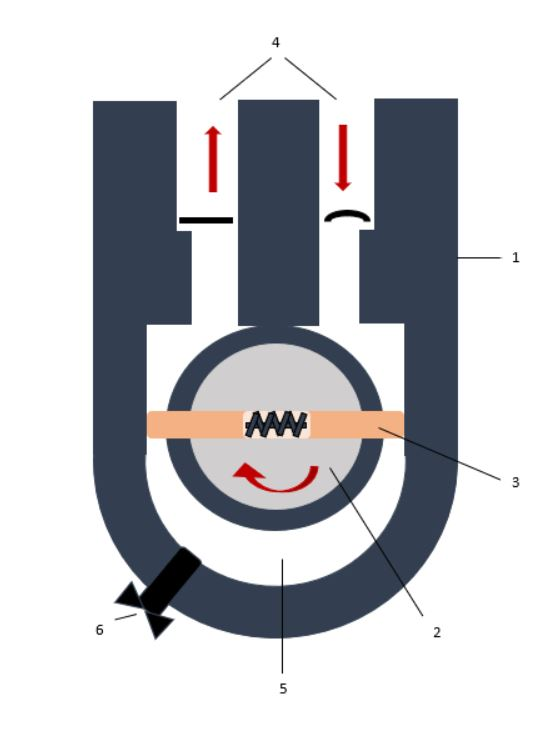
\includegraphics[height=0.35\textheight]{images/pumpe.jpg}
  \caption{Schematische Darstellung einer Drehschieberpumpe. Der innere Zylinder (2) rotiert nicht-zentral in dem Gehäuse (1). Der Drehschieber (3) rotiert und bildet abgetrennte Bereiche (z.B. (5)). Die Ein- und Auslassöffnungen (4) befinden sich am oberen Rand des Gehäuses, während unten ein Gasballast (6) durch Luftzufuhr die Kondensatbildung verhindert. \cite{pumpe}}
  \label{fig:pumpe}
\end{figure}

Die Versuchsdurchführung selbst gliedert sich in mehrere Teile.
Zunächst wird das verstärkte Signal um Oszilloskop gemacht und ein Bild aufgenommen. Für diese und die folgenden Messungen wird die Spannung des Surface-Barrier-Detektors auf $\SI{12}{\volt}$ geregelt und das Nachleuchten am Oszilloskop eingestellt, da das Signal teilweise deutlich schwankt.

Danach werden Messreihen aufgenommen, um die Foliendicke einer nach Herstellerangaben $\SI{2}{\micro\meter}$ dicken Goldfolie zu bestimmen. Dazu wird der Aufbau zunächst ohne eingebaute Folie so weit wie möglich evakuiert und die Pulshöhen am Oszilloskop in Abhängigkeit des Drucks zwischen ungefähr $100$ bis $\SI{200}{\milli\bar}$ gemessen. Die Messreihe wird für Drücke zwischen circa $100$ und $\SI{300}{\milli\bar}$ mit eingebauter Folie wiederholt. Dabei stehen sich Quelle und Detektor genau gegenüber, sodass die Strahlung die Goldfolie senkrecht trifft.

Die nächste Messaufgabe dient der Untersuchung des differenziellen Wirkungsquerschnitts für die $\SI{2}{\micro\meter}$ dicke Goldfolie. Dazu wird die Zählrate $I$ in Abhängigkeit des Streuwinkels $\theta$ gemessen. Zunächst wird am Zähler die Diskriminatorschwelle so eingestellt, dass bei Normaldruck und ausgebauter Goldfolie höchstens ein Ereignis pro Sekunde gemessen wird.

Danach wird auch für eine $\SI{4}{\micro\meter}$ dicke Goldfolie die Zählrate bei senkrechtem Einfall gemessen, der Vergleich mit der dünnen Goldfolie dient später der Untersuchung von Mehrfachstreuung.

Zuletzt wird für die beiden Goldfolien, eine Platin- und eine Bismutfolie für einen Winkel von $\SI{6}{\degree}$ die Zählrate gemessen, wobei die letzen beiden Folien eine Dicke von $\SI{2}{\micro\meter}$ bzw. $\SI{1}{\micro\meter}$ aufweisen. Damit soll später die Abhängigkeit des differenziellen Wirkungsquerschnitts von der Ordnungszahl $Z$ des Streumaterials untersucht werden.
